\documentclass[10pt,A4paper]{article}
\usepackage[
    a4paper,
    inner=2.5cm,
    outer=3cm
]{geometry}

\usepackage[utf8]{inputenc}
\usepackage[a4paper,
            inner=2.5cm,
            outer=3cm
            ]{geometry}
            
\usepackage{graphicx}% Include figure files
%\usepackage{dcolumn}% Align table columns on decimal point
\usepackage{bm}% bold math
\usepackage{color}
%\usepackage[subnum]{cases}
\usepackage{hyperref}
\usepackage[backend=biber,
            sorting=none,
%            citestyle=numeric-comp,
%\            bibstyle=ieee, 
            style=numeric-comp,
            hyperref=true,
            maxnames=2,
            url=false,
            isbn=false,
            eprint=false,
            date=year,
            doi=false,
            giveninits=true
            ]{biblatex}
\addbibresource{references.bib}
\usepackage{xpatch}
\xpatchbibmacro{journal+issuetitle}{%
\usebibmacro{journal}%
\setunit*{\addspace}%
}{%
\usebibmacro{journal}%
\setunit*{\addcomma\space}%
}{}{}

\renewbibmacro*{name:andothers}{% Based on name:andothers from biblatex.def
  \ifboolexpr{
    test {\ifnumequal{\value{listcount}}{\value{liststop}}}
    and
    test \ifmorenames
  }
    {\ifnumgreater{\value{liststop}}{1}
       {\finalandcomma}
       {}%
     \andothersdelim\bibstring[\emph]{andothers}}
    {}}


%\DeclareFieldFormat[article]{title}{#1}
\DeclareFieldFormat[article]{volume}{\textbf{#1}}
%\DeclareFieldFormat[book]{volume}{\textbf{#1}}

\renewcommand\newunitpunct{\addcomma\space}
\DefineBibliographyStrings{english}{%
page = {},
pages = {},
}

\renewbibmacro{in:}{\addcomma\addspace}

\renewbibmacro*{volume+number+eid}{%
\isdot
\printfield{volume}%
\setunit*{\addcomma\addspace}%
\iffieldundef{number}{}{%
\printtext{no\adddot\addnbthinspace}%
}%
\printfield{number}%
\setunit{\addcomma\space}%
\printfield{eid}}


\setlength{\tabcolsep}{1.3pt}
\usepackage{bm}
\usepackage{amsmath}
\usepackage{amssymb}
\usepackage{mathtools}
\usepackage{mathrsfs}
\usepackage[T1]{fontenc}
\usepackage{diagbox}
\usepackage{here}
\usepackage[dvipsnames]{xcolor}
\usepackage{lipsum}
\usepackage{multirow}
\usepackage{ctable} % for \specialrule command
\usepackage{array,booktabs}
\newcolumntype{M}[1]{>{\centering\arraybackslash}m{#1}}
\usepackage{subcaption}
\usepackage{float}
\restylefloat{table}
\numberwithin{equation}{section}

\newcommand{\mbP}{\textbf{P: }}
\newcommand{\mbC}{\textbf{C: }}
\newcommand{\mbx}{\mathbf{x}}
\newcommand{\mbm}{\mathbf{m}}
\newcommand{\mbp}{\mathbf{p}}
\newcommand{\mbu}{\mathbf{u}}
\newcommand{\mbF}{\mathbf{F}}
\newcommand{\mbH}{\mathbf{H}}
\newcommand{\cmtb}[1]{\textcolor{blue} {#1}}
\newcommand{\cmt}[1]{\textcolor{red} {[#1]}}

\title{Pool Model Paper}
\author{Polina Gaindrik}


\begin{document}
\maketitle

\tableofcontents

\newpage
%
%
%
%
% ================================================================================================
\section{Introduction}
Motivation: general, flexible approach for bacterial systems that allows easily modify the system depending on processes on different scales.
Allows us to describe the processes within populations using different bacterial states as well as interactions between different populations using ODEs.\\
%
%
Existing models in Predictive Microbiology (Primary Models)~\cite{perez-rodriguez_predictive_2012}:
\begin{itemize}
    \item An overview of primary models used in food science can be found in~\cite{van_boekel_kinetic_2008}.
    \item Baranyi-Roberts Model~\cite{baranyi_modeling_1993, baranyi_dynamic_1994}
    \item modified Gompertz
    \item Buchanan et al.: three-phase linear model for lag phase, exponential growth phase, and stationary phase~\cite{buchanan_when_1997}
    \item McKellar two-compartment model with bacteria in growing and non-growing state~\cite{mckellar_heterogeneous_1997}
    \item Inactivation models
\end{itemize}
%
Secondary models:
\begin{itemize}
    \item Polynomial models 
    \item Square Root-Type Models, e.g., Ratkowski for temperature~\cite{ratkowsky_relationship_1982}
    \item The Cardinal Parameter Model~\cite{zwietering_decision_1992}
\end{itemize}
%
%
Comprehensive reviews about competition/cooperation bacterial mechanisms: \cite{ghoul_ecology_2016, stubbendieck_bacterial_2016, hibbing_bacterial_2010, west_social_2007}\\
%
%
% ================================================================================================
\section{General Mathematical Formulation}
Consider the system consisting of $N$ species in $M$ different states.
In the general representation, the system can be described with the Ordinary Differential Equations (\acp{ode}) using a non-linear function $\mbF$:
\begin{equation}
   \dot{\mbx} = \mbF(\mbx, \mbm, \mbp, \mbu),
   \label{eq:model_ODE}
\end{equation}
where  $\mbx \in \mathbb{R}^{N}  \otimes \mathbb{R}^{M}$ is a vector describing bacterial count.
In matrix form it can be written as
\begin{equation}
    \mbx = \begin{pmatrix}
        x^1_1  & \dots & x^1_N  \\
        \vdots &       & \vdots \\
        x^M_1  & \dots & x^M_N  \\
            \end{pmatrix}
    \label{eq:model_bact}
\end{equation}
with $x_{j}^{i}$ describing the bacterial counts for species $i$ in state $j$.
$\mbu$ is the vector of different inputs of the model, e.g., temperature, pressure etc.
The vector $\mbm \in \mathbb{R}^{K}$ includes all variables corresponding to the microenvironment of the system which can be concentration of the inhibitors or activators:
\begin{equation}
    \dot{\mbm} = \mbH (\mbx, \mbm, \mbp, \mbu).
    \label{eq:model_microenv}
\end{equation}
Here function $\mbH$ is in general case also non-linear.\\
%
The advantage of the following formulation is its generality.
Depending on the knowledge about the system as well as the needed level of accuracy one can define an arbitrary number of states $M$ and control the complexity of the model.
Moreover, opposite to the already known Predictive Microbiology like Baranyi and Roberts one can easily change.\\
%
To calculate the bacterial count for one species $i$, we simply need to sum the tensor/vector $\mbx$ over all possible states:
\begin{equation}
    N_i = \sum_k \mbx_i^k.
\end{equation}
While the total bacterial count of all species of our system is
\begin{equation}
    N = \sum_i \sum_k \mbx_i^k.
\end{equation}
In the following section we demonstrate the application of this approach for different toy models describing the processes within and between bacteria communities.
%
%
%
%
% ================================================================================================
\section{One Species Modeling}
% ------------------------------------------------------------------------------------------------
\subsection{Three-Pool Model}
Consider for simplicity the system where only one bacteria species is present $N=1$.
The bacterial growth curves usually consist of different consecutive phases~\cite{buchanan_when_1997}.
At the beginning no increase in bacterial count is present and so-called lag-phase is observed.
This phenomenon appears due to adaptation of the microbial community, for example, to the new environmental conditions.
This so-called preparation to the exponential growth includes synthesys of the needed compounds, initiation of the transciption~\cite{rolfe_lag_2012} and poorly studied physiological and regulatory mechanisms~\cite{monod_growth_1949}.
After this, the succeeded in adaptation bacteria enter the exponential growth phase, where the process of cell division is directly happening.
When the nutrition is exhausted by the growing bacteria, the stationary state of the growth curve occurs.
In this state the cultures accumulate waste products of metabolic activity that leads to cell death of the bacteria.
At the same time dying cells release the nutritions for survivors to continue growing.
As a result the balance between the growing and dying processes leads to the constant with time bacterial count~\cite{navarro_llorens_stationary_2010}.
In the described simplified version of the real-life system three possible bacteria states are mentioned corresponding to which process is happening: adaptation, growth or death.
Motivated by this we divide a bacterial population into three pools (states) (~\ref{fig:SchematicRep}):
\begin{itemize}
\item $x^1_1 (t) = L(t)$: the fraction of the population in the lag phase
\item $x^2_1 (t) = G(t)$: the fraction of the population growing and dividing
\item $x^3_1 (t) = D(t)$: the fraction of the population undergoing cell death
\end{itemize}
Here the concentrations of the pools are components of our variable vector $\mbx (t) = (L(t), G(t), D(t))^T$.
\begin{figure}[t]
    \begin{center}
    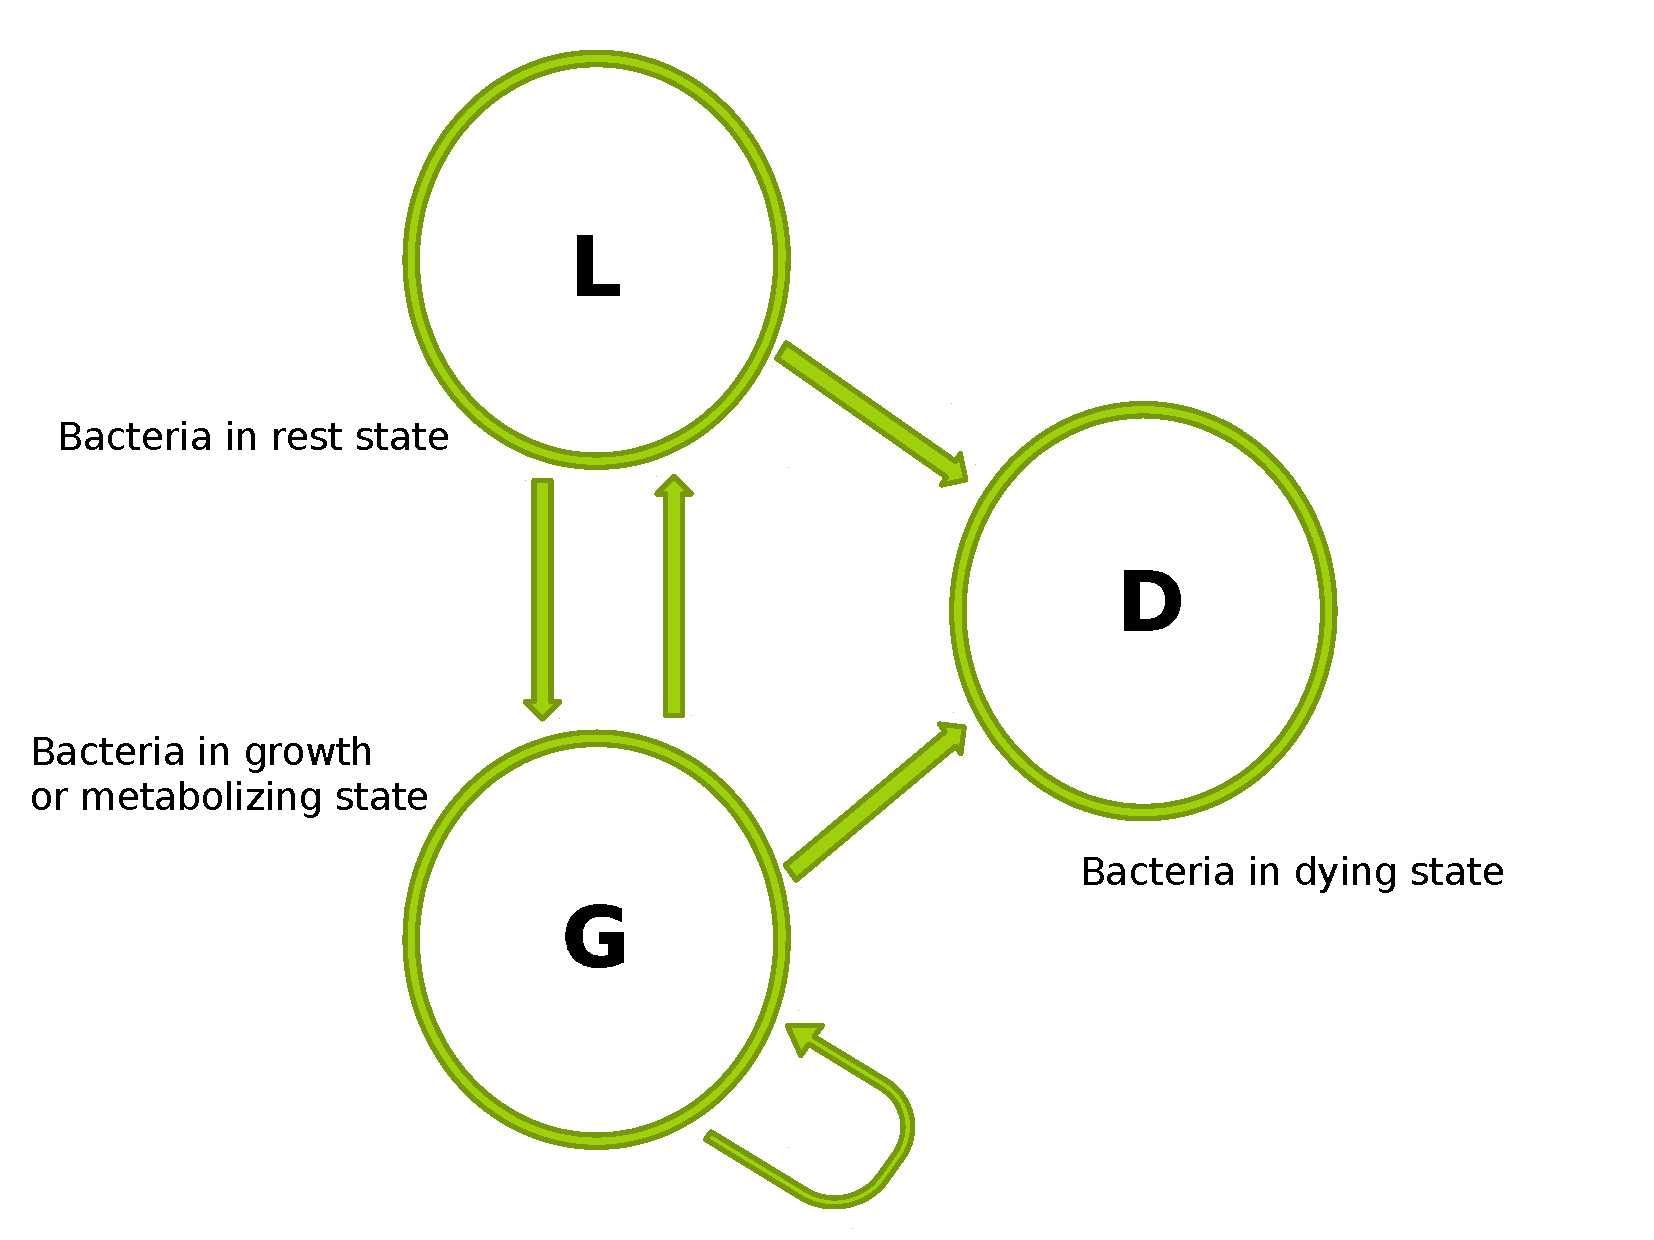
\includegraphics[width=0.6\textwidth]{Figures/TPM_fig.pdf}
    \caption{Schematic representation of exchange between three states or pools.}
    \label{fig:SchematicRep}
    \end{center}
\end{figure}
To determine the function $\mbF(\mbx, \mbm, \mbp, \mbu)$ consider the flows between different states.
The pools $G$ and $D$ are unidirectionally connected with the pool $L$.
For now, we assume for simplicity that there is no back flow between growth state $G$ and lag-state $L$.
The suggested model can be cast in the following reactions:
\begin{eqnarray}
    L &\stackrel{\lambda}{\longrightarrow} & G\\
    L &\stackrel{\mu}{\longrightarrow} & D\\
    G &\stackrel{\alpha}{\longrightarrow} & 2G\\
    G &\stackrel{\mu'}{\longrightarrow} & D\\
    D &\stackrel{\beta}{\longrightarrow} & \emptyset
\end{eqnarray}
Then the \acp{ode} describing such a model can be written as
\begin{equation}
\begin{cases}
    \dot{L} = -(\mu + \lambda) L\\
    \dot{G} = \lambda L + \alpha G - \mu' G\\
    \dot{D} = \mu  L + \mu' G- \beta D  
\end{cases}
\end{equation}
or in matrix form it shows the linear dependency
\begin{equation}
    \dot \mbx  = \begin{pmatrix}
        -(\mu + \lambda) & 0             & 0      \\
        \lambda          & \alpha - \mu' & 0      \\
        \mu              & \mu'          & -\beta 
    \end{pmatrix} \mbx .
\end{equation}
%
%
%
% ------------------------------------------------------------------------------------------------
\subsection{Resource Dependence}
Based on experimental observations, it was shown that the bacterial growth is strongly influenced by the limiting resource.
According to the works of Jacques Monod, in the system where all needed nutritients are in excess except for one the total growth is linear to the concentration of this limiting nutritient~\cite{monod_growth_1949}.
The control of the population density with respect to the available nutrition is implemented using cell communication process called quorum sensing.
Using release of the extracellular signalling molecules (autoinducers) it is possible to synchronize the gene expression of the whole group~\cite{ng_bacterial_2009}.
We would not dive into the processes of quorum sensing and try to keep it as simple as possible.
According to this, we aim to include a resource pool which is used by the growing bacteria using the second order kinetic reaction:
\begin{equation}
    G + R_0  \stackrel{\alpha_0}{\longrightarrow} 2G.
\end{equation}
Note that the pools $L$, $G$ and $D$ represent the number of bacteria (or number of bacteria per unit area/volume) while $R_0$ represents an abstract resource pool.
Let say $G=N_B/V$ and $[G]=1/V$, where $N_B$ is the number of bacteria and $V$ is the volume.
Then $R_0=N_R/V$ and $[R_0]=1/V$, where $N_R$ is the number of resource molecules (or any appropriate unit, e.g., mol).
Then $[\alpha_0]=V/s$, $[N_t]=1/V$, and $[\alpha]=1/s$.
For homogeneous densities it is equivalent to consider the total amount, i.e., multiplying $L$ and $G$ by the volume.
In this case $[L]=[G]=[N_t]=1$.
For simplicity, we rather make a transition to the dimensionless constant $\alpha:=\alpha_0 N_t$ and dimensionless resource pool $R(t) = R_0 / N_t$ ($0 \leqslant R \leqslant 1$).
Here the full capacity of the resource pool $N_t$ was used as a scaling constant.
In this case the growth term can be simply written as $\alpha G R$ and the model is fully formulated in the following way:
\begin{eqnarray}
    \dot \mbx  &=& \mbF(\mbx, \mbm, \mbp, \mbu) = \begin{pmatrix}
        -(\mu + \lambda) & 0               & 0      \\
        \lambda          & \alpha R - \mu' & 0      \\
        \mu              & \mu'            & -\beta 
    \end{pmatrix} \mbx\\
    \dot \mbm &=& \mbH (\mbx, \mbm, \mbp, \mbu) = -\frac{\alpha}{N_t} R G.
\end{eqnarray}
%
Such model can be simplified by exploiting that limitation of the resource pool also limits the total bacterial count of the system:
\begin{equation}
    R = 1 - \frac{L+G+D}{N_t}
\end{equation}
and, hence, the full system can be written as
\begin{equation}
    \begin{cases}
        \dot{L} = -(\mu + \lambda) L\\
        \dot{G} = \lambda L + \alpha G\left(1-\frac{L+G+D}{N_t}\right)-\mu' G\\
        \dot{D} = \mu  L + \mu' G- \beta D 
        \label{eq:3pool_resource} 
    \end{cases}.
\end{equation}
Rewriting the equations above, we get the following non-linear system:
\begin{equation}
    \dot \mbx = \begin{pmatrix}
        -(\mu + \lambda) & 0       & 0 \\
         \lambda         & \alpha  & 0 \\
         \mu &  \mu'& - \beta 
    \end{pmatrix} 
    \mbx + \frac{\alpha}{N_t} x^2 \sum_i^3 x^i \begin{pmatrix} 0 \\ 1 \\ 0  \end{pmatrix}.
\end{equation}
Here the first term is the linear part and the second term define the quadratic behavior of the system.
\begin{figure}[t]
    \begin{center}
    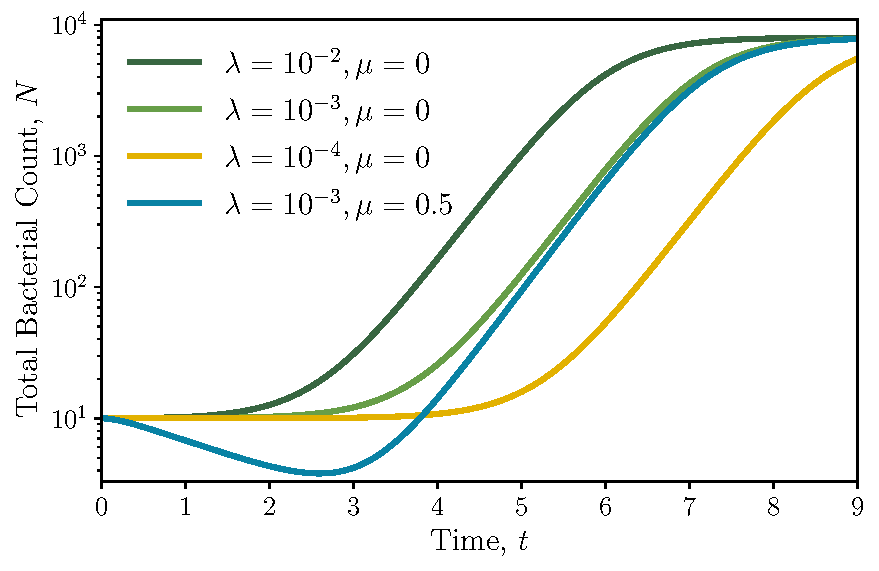
\includegraphics[width=0.6\textwidth]{Figures/pool_model_3pools_resource.pdf}
    \caption{
        The time dependence of the total bacterial count $N(t) = \sum_i \sum_k \mbx_i^k = L(t) + G(t) + D(t)$ is obtained as a sum of bacteria in all states.
        All curves were calculated using the model (\ref{eq:3pool_resource}) with parameters $\alpha=2.5$, $\mu'=0.5$ and $\beta=5$.
        The blue curve shows significant dip in behavior of the system where the death of the bacteria is present $\mu = 0.5$.
        Other curves show the case of no bacteria dying $\mu=0$ and represent different length of lag phases:
        short $\lambda=10^{-2}$ (dark green), intermediate $\lambda=10^{-3}$ (light green) and long one $\lambda=10^{-4}$ (yellow).
    }
    \label{fig:3pool_resource_plots}
    \end{center}
\end{figure}
The resulting growth curves for the three pool case are presented in Figure~\ref{fig:3pool_resource_plots}.
Here we can see that the value of the transition constant $\lambda$ determines how long the bacteria is in lag-phase.
The larger is the rate the shorter is the lag-time.
Moreover, by including the bacteria flow to the death pool we can diversify the shape of the growth curve allowing the decrease of the bacterial count.
%
%
%
% ------------------------------------------------------------------------------------------------
\subsection{Lag-time Estimation}
Note that one could further simplify this model to a two pool or state model by omitting the pool $D$ and removing cells with rate $\beta$ directly from pool $L$.
The relevant question here is whether cells in the pool $D$ still contribute to the limitation of the resources by, e.g., occupying space or consuming important nutrients.
If yes, the three pool model would be advantageous, if not the two pool model is sufficient with the advantages of having one parameter less.\\
%
The dynamics of the three pool model can be captures by the coupled system of ordinary differential equations (the two pool model can be achieved by setting $D\equiv 0$ and replacing $\mu$ with $\beta$):
to be solved with the initial conditions $L(0)=N_0$, $G(0)=0$, and $D(0)=0$, where $N_0$ is the initial bacterial population.
$N_t$ denotes the maximal size of the total bacterial population due to environmental limitations (Figure \ref{fig:3pool_resource_plots}).
For $\mu'=0$ the equations for $L$ and $D$ can be readily integrated resulting in:
\begin{equation}
    \begin{cases}
        L(t) = N_0 e^{-(\mu+\lambda)t}\\
        D(t) = N_0 \mu e^{-\beta t}\frac{1-e^{-(\mu+\lambda-\beta)t}}{\mu+\lambda-\beta}
    \end{cases}.
\end{equation}
For constant parameters $\mu$, $\lambda$, and $\beta$ the integrals for $L$ and $D$ can be put into the differential equation for $G$.
However, for time dependent parameters, e.g., for a dependence on a non-static, dynamic temperature, it appears to be not advantageous to use the analytical results for $L$ and $D$ and work instead with all three equations for $L$, $G$, and $D$.
It is interesting to see what type of equations result for the total bacterial population $N=L+G+D$:
\begin{equation}
    \begin{cases}
        \dot{G} = \lambda L + \alpha G\left(1-\frac{N}{N_t}\right)\\
        \dot{N} = - \beta D + \alpha G\left(1-\frac{N}{N_t}\right)
    \end{cases}
\end{equation}
with the initial conditions $G(0)=0$ and $N(0)=N_0$. 
These equations have a clear interpretation, are derived from simple principles, and are different from the popular Barayni-Roberts and modified-Gompertz models.
A notable difference is that the growth rate $\alpha$ is time independent.
For the functions $L$ and $D$ it holds: $\lim_{t\to\infty} L(t) = \lim_{t\to\infty} D(t) = 0$.
It follows immediately that $\lim_{t\to\infty} G(t) = N_t$.
The equation exhibit a lag phase and an initial drop due to cell death.
To find a substantial initial drop one needs $\beta \mu \gg \alpha \lambda$.
The lag time $t_L$ can be approximated by the time at which half of the initial population is in the growth phase, i.e., $N_0=2G(t_L)$.
Assuming $L\ll N_t$ we can ignore the non-linear term in the equation for $G$, which gives rise to:
\begin{eqnarray}
    1&=& 2\int_0^{t_L} \lambda L(t)e^{\alpha(t_L-t)}dt\\
    1  &=& 2\lambda e^{\alpha t_L}\frac{1-e^{-(\mu+\lambda+\alpha)t_L}}{\mu+\lambda+\alpha}.
\end{eqnarray}
For $\alpha > \mu+\lambda$ $t_L$ can be approximated by:
\begin{eqnarray}
    t_L &\approx& -\frac{1}{\alpha}\ln\left(\frac{2\lambda}{\mu+\lambda+\alpha}\right).
\end{eqnarray}
The lag time $t_L$ diverges very slowly, logarithmically with $\lambda\to 0$.
%
%
%
% ------------------------------------------------------------------------------------------------
\subsection{Back flow from Growth to Lag pool}
Due to its life in rather unfavorable conditions bacteria developed different surviving mechanisms, one of which is adapting their metabolism and transitioning into dormant state.
By definition dormancy in bacteria is a reversible state where cell continue living with low metabolic activity while the cell division stops~\cite{kaprelyants_dormancy_1993}.
This survival strategy can appear in response to different external stresses, e.g., nutritient deficiency, temperature stress or extreme fluctuations of environment parameters.
And after "difficult times" bacteria, also called viable but non-culturable (VBNC), can continue cell division~\cite{kell_viability_1998}.
The models including transition of bacteria to the dormant state were proposed and studied by Bär \etal~\cite{bar_modelling_2002} and Jones and Lennon~\cite{jones_dormancy_2010}.
%
\cmt{So now is it better to use flow to dormancy instead?}
%
We explore now the idea that under certain conditions, as sudden change in the environment, part of the population $G$ will enter a lag-phase, i.e., there is a back-flow from $G$ to $L$.
\begin{eqnarray}
    L &\stackrel{\lambda}{\longrightarrow} & G\\
    L &\stackrel{\mu}{\longrightarrow} & D\\
    G &\stackrel{\alpha}{\longrightarrow} & 2G\\
    G &\stackrel{\gamma(t)}{\longrightarrow} & L\\
    D &\stackrel{\beta}{\longrightarrow} & \emptyset
\end{eqnarray}
The rate $\gamma(t)$ depends on the rate of change of the environment.
Stronger and quicker changes will lead to a higher rate $\gamma$.
%
%
% ................................................................................................
\subsubsection{Maxwell type of stress - strain relation}
One of the reasons of the dormant state appearance can be also the temperature shift~\cite{oliver_viable_1995}.
Moreover, the rapid shift in temperature is associated with the appearance of an additional lag phase~\cite{zwietering_modeling_1994}.
To model it we propose a kind of viscoelastic Maxwell type of stress-strain relation and write down the ordinary differential equation for $\gamma$ to be:
\begin{eqnarray}
    \dot{\gamma} &=& \Gamma \left |\dot{T}\right |-\delta \gamma.
\end{eqnarray}
We assumed that the direction of the temperature change does not matter, i.e., a change from $T=2$ to $T=12$ has the same effect as a change from $T=14$ to $T=4$.
$\Gamma$ is a scaling factor and $\delta$ is the relaxation time for the temperature disturbance.
Integration of this equation yields (with $\gamma(0)=0$):
\begin{eqnarray}
    \gamma(t) &=& \Gamma \int_0^t \left |\dot{T}(t^{\prime})\right |e^{-\delta (t-t^{\prime})}dt^{\prime}.
\end{eqnarray}
After some manipulation of this equation we find:
\begin{eqnarray}
    \gamma(t) &=& \Gamma\delta\left |\left[T[t]-T[0]e^{-\delta t}-\delta \int_0^t T(t^{\prime})e^{-\delta (t-t^{\prime})}dt^{\prime}\right]\right |.
\end{eqnarray}
This representation of the rate $\gamma(t)$ has the advantage that it only involves $T(t)$ and does not require the calculation of the derivative of $T$.
If $T$ exhibits $n$ temperature jumps, one finds:
\begin{eqnarray}
    \gamma(t) &=& \Gamma\sum_{i=1}^n \left |\Delta T_i \right |\theta(t-t_i)e^{-\delta(t-t_i)}.
    \label{eq:gamma_tempshift}
\end{eqnarray}
%
The ordinary differential equations for the pool model with environmental-shock based back-flow read:
\begin{equation}
    \begin{cases}
    \dot{L} =\gamma(t) G - (\mu + \lambda) L\\
    \dot{G} = \lambda L -\gamma(t) G + \alpha G\left(1-\frac{L+G+D}{N_t}\right)\\
    \dot{D} = \mu  L - \beta D
    \label{eq:ODE_tempshift}
    \end{cases}
\end{equation}
\begin{figure}[t]
    \begin{center}
    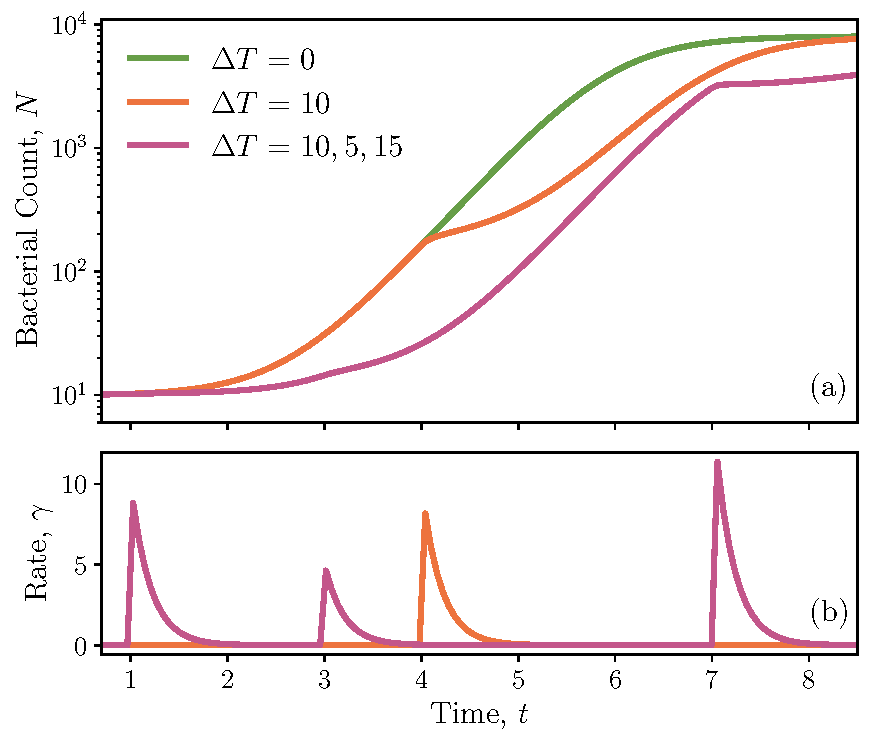
\includegraphics[width=0.6\textwidth]{Figures/pool_model_3pools_resource_tempshift.pdf}
    \caption{
        (a) The time dependence of the total bacterial count $N$ for the model including the back-flow to the lag phase due to temperature stress~(\ref{eq:ODE_tempshift}).
        (b) The value of the corresponding back-flow rate $\gamma$ calculated according to (\ref{eq:gamma_tempshift}).
        The curves represent no temperature shift (green), one temperature jump $\Delta T = 10$ at time $t=4$ (orange)
        and the series of different temperature shifts of value 10, 5 and 15 at the time points 1, 3 and 7, respectively (rose).
        The parameters of the back-flow rate are $\Gamma=1$ and $\delta=5$.
        The other model parameters are $\alpha=2.5$, $\mu'=0.5$, $\beta=5$, $\lambda=10^{-2}$, $\mu = 0$ for each curve.
    }
    \label{fig:TempJump}
    \end{center}
\end{figure}
The effect of the temperature shift on the total bacterial count can be shown in Figure~\ref{fig:TempJump}.
After the rapid temperature increase, the growth slows down till the bacteria that transitioned back to lag-phase go again to growth pool.
If the shift happened rather early in time, when most of the bacteria were in lag-phase, the effect is not noticeable.
\newpage
%
%
%
% ================================================================================================
\section{Interaction between species}
As it was mentioned above, bacteria usually coexist in large multispecies interacting communities whose growth is vastly determined by the developed survival mechanisms.
These survival mechanisms mostly aim to secure as much available nutrition which lead to competitive strategies or, if it is advantageous, cooperative ones~\cite{hibbing_bacterial_2010, stubbendieck_bacterial_2016}.
Further we show that the model can be readily extended to the systems with more than one bacterium and describe more complex relationships between species. 
%
%
%
% ------------------------------------------------------------------------------------------------
\subsection{Resource Competition}
One on the ways to describe competition between bacteria populations is as a function of limiting resource ratio~\cite{tilman_resource_1977, smith_effects_2002}.
To describe such a situation we consider for simplicity only one common limiting resource pool.
The simplest pool model for bacterial species $A$ and $B$ encompassing lag-phases, growth-phases and a common resource pool is given by (no back-flow to the lag-pool):
\begin{equation}
    \begin{cases}
        \dot{L}_A = - \lambda_A R L_A\\
        \dot{L}_B = - \lambda_B R L_B \\
        \dot{G}_A = \lambda_A R L_A +\alpha_A R G_A\\
        \dot{G}_B = \lambda_B R L_B +\alpha_B R G_B\\
        \dot{R} =-\frac{\alpha_A}{N_t} R G_A-\frac{\alpha_B}{N_t} R G_B
    \end{cases}
    \label{eq:model_2sp_resource_comp}
\end{equation}
This system of equations defines the microenvironment $\mbm$ and bacteria state matrix $\mbx$ as
\begin{equation}
    \mbm = R, \hspace{1cm}
    \mbx = \begin{pmatrix}
        L_A & L_B \\
        G_A & G_B 
    \end{pmatrix}.
\end{equation}
We again rescaled the resource pool with $N_t$ and find
\begin{eqnarray}
\label{eq:Resource}
R &=&1-\frac{L_A+G_A+L_B+G_B}{N_t}
\end{eqnarray}
Inserting Eq.~\ref{eq:Resource} into Eqs.~\ref{eq:model_2sp_resource_comp} yields:
\begin{eqnarray*}
    \dot{L}_A &=& - \lambda_A  L_A + \frac{\lambda_A}{N_t}\left(L_A+G_A+L_B+G_B\right)L_A\\
    \dot{L}_B &=& - \lambda_B L_B + \frac{\lambda_B}{N_t}\left(L_A+G_A+L_B+G_B\right)L_B \\
    \dot{G}_A &=&  \lambda_A  L_A - \frac{\lambda_A}{N_t}\left(L_A+G_A+L_B+G_B\right)L_A +\alpha_A G_A - \frac{\alpha_A}{N_t}\left(L_A+G_A+L_B+G_B\right)G_A\\
    \dot{G}_B &=&  \lambda_B L_B - \frac{\lambda_B}{N_t}\left(L_A+G_A+L_B+G_B\right)L_B  +\alpha_B G_B -\frac{\alpha_B}{N_t}\left(L_A+G_A+L_B+G_B\right)G_B
\end{eqnarray*}
which has the structure of a \ac{glv} expanded with different internal states for one species.
As one can see in Figure~\ref{fig:2pool_resource_2sp} even without direct interaction between species the bacterial growth was inhibited due to the limitation of the resource.
Here species $A$ has a longer lag-phase than $B$ but the exponential growth of $A$ is stronger than the one that bacteria $B$ experiences.
As a result, species $A$ was able to suppress species $B$ consuming the larger amount of nutritient and reaching larger bacterial count at the end.
\begin{figure}[H]
    \begin{center}
    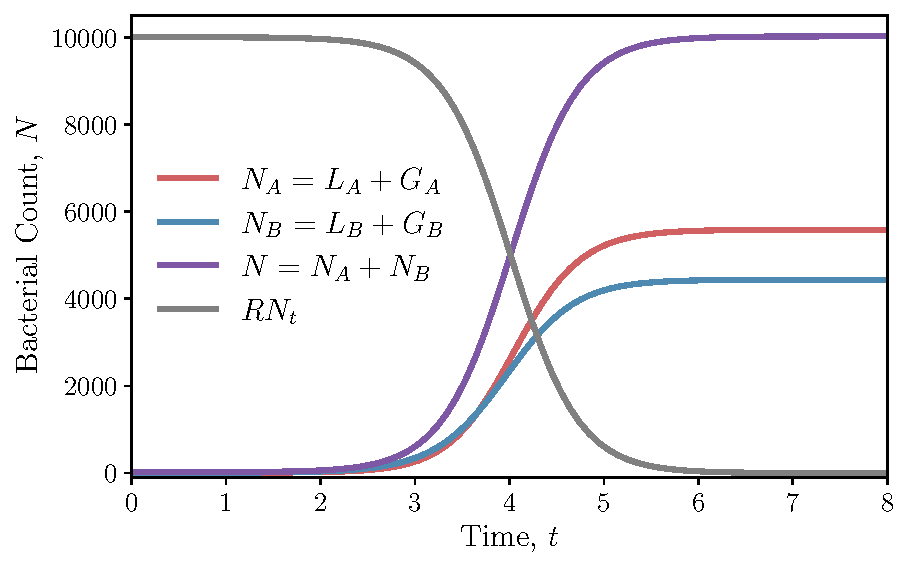
\includegraphics[width=0.6\textwidth]{Figures/pool_model_2pools_resource_competition.pdf}
    \caption{
        The competition of the two bacterial species due to the common limiting resource calculated using Eq.~(\ref{eq:model_2sp_resource_comp}).
        The red curve describes the growth of the bacteria $A$ ($N_A = \sum_{k} x_A^k = L_A+G_A$) with model parameters $\lambda_A=10^{-2}$, $\alpha_A=3.0$.
        The blue curve describes the growth of the bacteria $B$ ($N_B = \sum_{k} x_B^k = L_B+G_B$) with model parameters $\lambda_B=5\cdot 10^{-2}$, $\alpha_B=2.5$.
        The purple line shows the total bacterial count of the system  $N(t)=\sum_i\sum_k\mbx_i^k=N_A+N_B$.
        The gray line denotes the dynamic of the resource pool scaled with its capacity $N_t=10^4$.
    }
    \label{fig:2pool_resource_2sp}
    \end{center}
\end{figure}
%
In order to get the commonly used form of the \ac{glv}, we need to simply eliminate of the bacterial states by setting $L_A=L_B=0$:
\begin{equation}
    \begin{cases}
    \dot{G}_A = \alpha_A G_A\left(1 - \frac{G_A}{N_t}\right) - \frac{\alpha_A}{N_t}G_AG_B\\
    \dot{G}_B = \alpha_B G_B\left(1-\frac{G_B}{N_t}\right) -\frac{\alpha_B}{N_t}G_AG_B. 
    \label{eq:LV_simple}
    \end{cases}
\end{equation}

%
Equations (\ref{eq:LV_simple}) are basically competitive Lotka-Volterra equations that are widely used in ecological studies and show the principle of competitive excursion.
That principle claims that two species in competition for the same resource cannot coexist~\cite{wangersky_lotka-volterra_1978}.
In previous studies it was shown that \ac{glv} equations with one bacterial state can be sucessfully applied to predict the microbial community dynamics, determine different types of the pairwise interspecies interactions~\cite{dedrick_when_2023, stein_ecological_2013, venturelli_deciphering_2018, hoffmann_power_2007}.
In food studies the \ac{glv} was applied by Mounier \etal~\cite{mounier_microbial_2008} to study interactions of six bacteria species influenced by yeast omissions in cheese.
Cauchie \etal~\cite{cauchie_modeling_2020} applied Lotka-Volterra model to study the three-species system of the bacteria majorly present in minced pork meat.\\
%
However, in contrast to the classical Lotka-Volterra approach, the introduced pool model allows for far more flexibility in tuning properties of the bacterial interactions within and between species.
%
%
%
% ------------------------------------------------------------------------------------------------
\subsection{Interspecies Competition}
However, except the inhibition due to resource competition, bacteria developed different others active competition mechanisms.
One of the examples of such mechanisms is a production of the antimicrobial compounds, inhibitors or toxins~\cite{wloch-salamon_effect_2008, chao_structured_1981}.
On the other hand, some bacteria can produce public goods, the compounds that benefit growth of other species.
In this way, can suppress the non-preferred species by helping their competitors~\cite{hibbing_bacterial_2010}.
%
%
% ................................................................................................
\subsubsection{Toxins Production}
To introduce active competitive mechanisms, we extend our model with one of the species producing the toxic compounds $T$ during its growth:
\begin{eqnarray}
    \dot{T} &=& \mathcal{F}(R,G).
\end{eqnarray}
The function $\mathcal{F}$ denotes the model for the toxin production rate.
It can be, for example, the accumulation of the bacteria waste which is responsible for the spoilage of food products and affecting another species in negative way.
Consider the system for two species competing for resource $R$ with the production of the toxin $T$ by species $B$.
Assume that the toxin causes the death of the species $A$ with rate $\mu$.
Then the full \ac{ode} system is
\begin{equation}
    \begin{cases}
        \dot{L}_A = - \lambda_A R L_A\\
        \dot{L}_B = - \lambda_B R L_B \\
        \dot{G}_A = \lambda_A R L_A + \alpha_A R G_A - \frac{\mu}{\kappa N_t} T G_A\\
        \dot{G}_B = \lambda_B R L_B + \alpha_B R G_B\\ 
        \dot{R} = -\frac{\alpha_A}{N_t} R G_A-\frac{\alpha_B}{N_t} R G_B\\
        \dot{T}_{B}^{1,2} = \mathcal{F}^{1,2} (R, G_B) \\
    \end{cases}.
    \label{eq:model_2sp_toxin}
\end{equation}
%
Where we consider two possible models of the toxin production:
\begin{eqnarray}
    \mathcal{F}^1(R,G)&=&\kappa G_B\\
    \mathcal{F}^2(R,G)&=&\kappa\alpha_B R G_B.
\end{eqnarray}
Here $\kappa$ is the toxin production rate.
The difference between the two toxin production models for resulting solution of the \acp{ode} is presented in Figure~\ref{fig:2pool_2sp_toxin}.
%
%
\begin{figure}[H]
    \begin{center}
    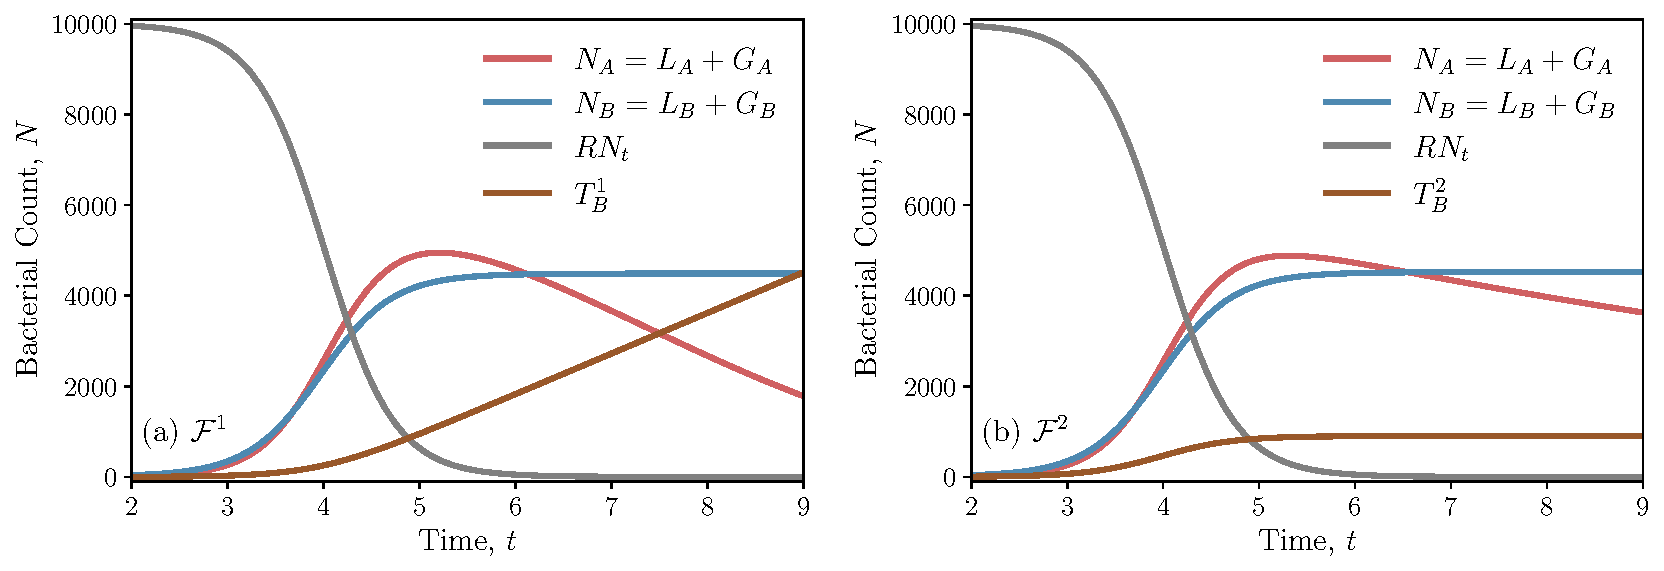
\includegraphics[width=1.\textwidth]{Figures/pool_model_2pools_toxin.pdf}
    \caption{
        The two species system competing for the common nutritient $R$ with production of the toxin $T_B$ (brown line) calculated using Eq.~(\ref{eq:model_2sp_toxin}).
        The growing bacteria $B$ produces toxin $T_B$ (a) constantly $\dot{T}_B^1 = \mathcal{F}^1 = \kappa G_B$ or (b) only during growth process $\dot{T}_B^2 = \mathcal{F}^2 = \kappa \alpha_B R G_B$ with 
        production rate $\kappa=0.2$.
        The toxin $T_B$ causes the cell death of bacteria $A$ with rate constant $\mu = 0.2$.
        The red curve describes the growth of the bacteria $A$ ($N_A = \sum_{k} x_A^k = L_A+G_A$) with model parameters $\lambda_A=10^{-2}$, $\alpha_A=3.0$.
        The blue curve describes the growth of the bacteria $B$ ($N_B = \sum_{k} x_B^k = L_B+G_B$) with model parameters $\lambda_A=5\cdot 10^{-2}$, $\alpha_A=2.5$.
        The gray line denotes the dynamic of the resource pool scaled with its capacity $N_t=10^4$.
    }
    \label{fig:2pool_2sp_toxin}
    \end{center}
\end{figure}
%
Model $\mathcal{F}^1$ results in toxin concentration $T_B^1(t)=\kappa\int_{t_0}^tG(t')dt'$.
That means that as long as there are bacteria in the growth phase $G_B>0$ toxin is produced, no matter whether the total bacterial count $N_B$ is still growing.
On the other hand, model $\mathcal{F}^2$ results in toxin accumulation in steady state $T_B^{2s}=\lim_{t\to\infty}T_B^2(t)=\kappa(N_t-N_0)$.
To see this we note $\dot{T}_B^2=\kappa(\dot{L_B}+\dot{G_B})$, which yields: $T_B^2(t)=\kappa(L_B(t)+G_B(t)-N_{B0})$ where we used $T_B^2(0)=G_B(0)=0$, $L_B(0)=N_{B0}$.
This model assumes that toxin is only produced when the total bacterial grow and divide, hence, the total bacterial count $N_B$ increases.
%
%
% ................................................................................................
\subsubsection{Mutual Inhibition}
Another special case of the species competition is when the produced toxin does not cause the death of the bacteria but rather inhibit its growth.
Such situation with 2 bacteria species, limiting resource and produced inhibitor was modeled, e.g., by Lenski and Hattingh~\cite{lenski_coexistence_1986}.
In our case, we would like to look at rather simplified case reducing the number of variables of the system.
The easiest way to introduce inhibition of species $A$ by species $B$ is via a growth rate of species $A$ depending on the abundance of species $B$.
For sake of simplicity we ignore the lag pool and write for a mutual inhibition:
\begin{eqnarray}
    \dot{G}_A &=& \mathcal{B}_A(G_B)G_A\left(1 - \frac{G_A+G_B}{N_t}\right)\\
    \dot{G}_B &=& \mathcal{B}_B(G_A) G_B\left(1-\frac{G_A+G_B}{N_t}\right).
\end{eqnarray}
The function $\mathcal{B}_{A/B}$ captures the inhibiting effects effectively.
It is straight forward to make the mechanism of inhibition more explicit by, e.g., introducing a toxin pool.
One possible choice for $\mathcal{B}$ is:
\begin{eqnarray}
    \mathcal{B}(G)&=&\frac{\alpha}{1+KG}. 
\end{eqnarray}
This corresponds to the case $T\sim G$, where $T$ is the toxin produced.
If the toxin accumulates one needs to replace $G$ by $\int G dt$. Keeping it simple yields:
\begin{eqnarray}
    \dot{G}_A &=& \frac{\alpha_A G_A}{1+K_BG_B}\left(1 - \frac{G_A+G_B}{N_t}\right)\\
    \dot{G}_B &=& \frac{\alpha_B G_B}{1+K_AG_A}\left(1-\frac{G_A+G_B}{N_t}\right). 
\end{eqnarray}
One can distinguish two limiting cases: {\it i}) $K_{A/B}\ll N_t$ and {\it ii}) $K_{A/B}\gg N_t$.
In the first case the inhibition is of minor importance and could be ignored.
In the latter case one can simplify the equations, given $N_A$ and $N_B$ are non-zero:
\begin{eqnarray}
\label{Mut_Inhib}
    \dot{G}_A &=&\tilde{\alpha}_A\frac{G_A}{G_B}\left(1 - G_A-G_B\right)\\
    \dot{G}_B &=& \tilde{\alpha}_B\frac{G_B}{G_A}\left(1-G_A-G_B\right).
\end{eqnarray}
We introduced the rescaled growth rates $\tilde{\alpha}_A=\alpha_A/(N_tK_B)$ and $\tilde{\alpha}_B=\alpha_B/(N_tK_A)$. Note that $[\tilde{\alpha}]=\mathrm{s}^{-1}$.
Rescaling time with $\tilde{\alpha}_A$ and defining the dimensionless parameter
\begin{equation}
    \psi = \tilde{\alpha}_B/\tilde{\alpha}_A = \frac{K_B\alpha_B}{K_A\alpha_A}
\end{equation}
results in: 
\begin{equation}
    \begin{cases}
    \dot{G}_A =\frac{G_A}{G_B}\left(1 - G_A-G_B\right)\\
    \dot{G}_B =\psi\frac{G_B}{G_A}\left(1-G_A-G_B\right). 
    \end{cases}
    \label{eq:2sp_1pool_inhibit_unitless}
\end{equation}
We can separate three cases (see Figure~\ref{fig:1pool_2sp_inhibit}):
\begin{eqnarray}
    \psi&=&1:\quad\text{A and B are equivalent}\\
    \psi&>&1:\quad\text{Species B growth faster and/or inhibits A stronger}\\
    \psi&<&1:\quad\text{Species A growth faster and/or inhibits B stronger}
\end{eqnarray}
%
\begin{figure}[H]
    \begin{center}
    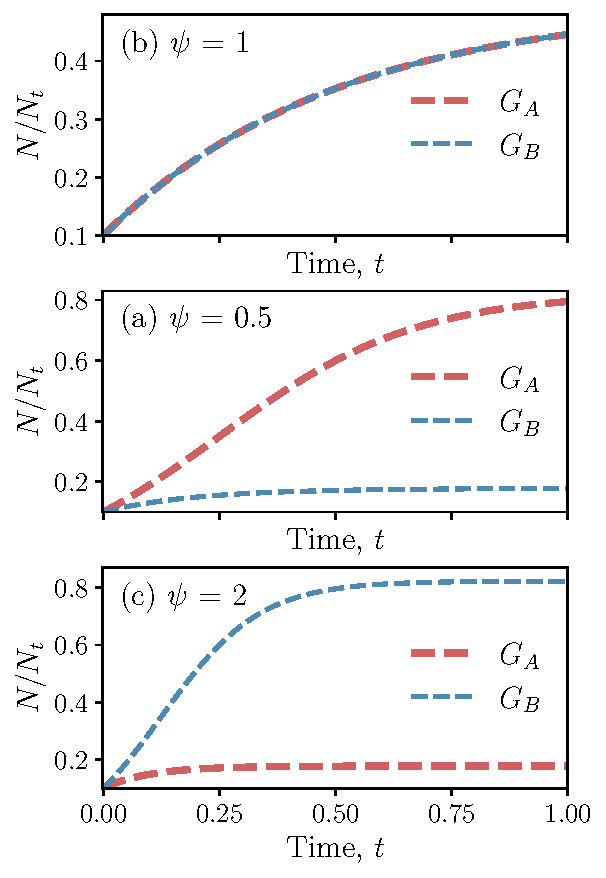
\includegraphics[width=0.5\textwidth]{Figures/pool_model_1pool_inhib.pdf}
    \caption{
        The two-species system mutually inhibiting each other is defined with equations~(\ref{eq:2sp_1pool_inhibit_unitless}).
        Here the red lines describes the evolution of the species $A$ and blue lines correspond to species $B$.
        The relation between inhibition strength of species $B$ and $A$ are defined by control parameter value (a) $\psi$ = 1, (b) $\psi$ = 0.5 or (c) $\psi$ = 2.
    }
    \label{fig:1pool_2sp_inhibit}
    \end{center}
\end{figure}
%
%
%
% ------------------------------------------------------------------------------------------------
\subsection{Interspecies Cooperation}
On the other hand, one can also observe some cooperative behaviors between species in case when it facilitates the competition with others.
It happens if bacteria species as a result of their metabolism produce the compounds that are beneficial for the growth of each other, so-called public goods.
Quite often it happens between the species that are close relatives or clonal populations and such process is called kin selection \cite{west_social_2007}.
Furthermore, Sometimes neighbors can benefit from a certain behavior without expressing it by itself, so-called 'social cheaters'~\cite{rainey_evolution_2003}.
%
%
The benefit, or mutual activation, of the two species from the presence of the other can be simply introduced by mathematical functions.
For sake of clarity we omit again the lag pool and write:
\begin{eqnarray}
    \dot{G}_A &=& \mathcal{B}_A(P_B,R)G_A\\
    \dot{G}_B &=& \mathcal{B}_B(P_A,R)G_B\\
    \dot{R} &=&-\mathcal{B}_A(P_B,R)G_A-\mathcal{B}_B(P_A,R)G_B\\
    \dot{P}_A &=& \mathcal{F}_A(R,G_A)\\
    \dot{P}_B &=& \mathcal{F}_B(R,G_B).
\end{eqnarray}
$P_A$ and $P_B$ denote the substance produced by species A and B, respectively.
The functions $\mathcal{B}_A(P_B,R)$ and $\mathcal{B}_B(P_A,R)$ capture the resource dependent growth.
Setting $\mathcal{B}_A(P_B,R)=\alpha_A P_BR$, $\mathcal{B}_B(P_A,R)=\alpha_B P_A R$, $\mathcal{F}_A(R,G_A)=\kappa_A RG_A$, $\mathcal{F}_B(R,G_B)=\kappa_B RG_B$, rescaling $G_A$, $G_B$, and $P_B$ with $N_t$, $P_A$ with $\kappa_A/\alpha_A$, time with $\alpha_AN_t^2$, defining $\psi=\kappa_A\alpha_B/(\alpha_A^2N_t)$, and $\phi=\kappa_B/(\alpha_A N_t)$ results in:
\begin{equation}
    \begin{cases}
    \dot{G}_A = P_B G_A\left(1 - G_A-G_B\right)\\
    \dot{G}_B = \psi P_A G_B\left(1 - G_A-G_B\right)\\
    \dot{P}_A = G_A\left(1 - G_A-G_B\right)\\
    \dot{P}_B =\phi G_B\left(1 - G_A-G_B\right)
    \end{cases}.
    \label{eq:1pool_2sp_cooper}
\end{equation}
%
The solution of the system~\ref{eq:1pool_2sp_cooper} is presented in Figure~\ref{fig:1pool_2sp_cooper}.
Here we can see that if $\psi=1$ and $\phi=1$ (see Figure~\ref{fig:1pool_2sp_cooper}a) the production of the public goods of the two species is happening with the same rate as well as the growth of bacteria.
Increasing the production rate of the public good produced by species $B$ (see Figure~\ref{fig:1pool_2sp_cooper}b) causes increasing the growth of species $A$ that profit from the presence of $B$.
On the other hand, choosing $\psi=2$ (see Figure~\ref{fig:1pool_2sp_cooper}c), we increase the profit that species $B$ has from public goods $P_A$.
That indirectly leads to larger amount of $P_B$ produced by species $B$.
\begin{figure}[H]
    \begin{center}
    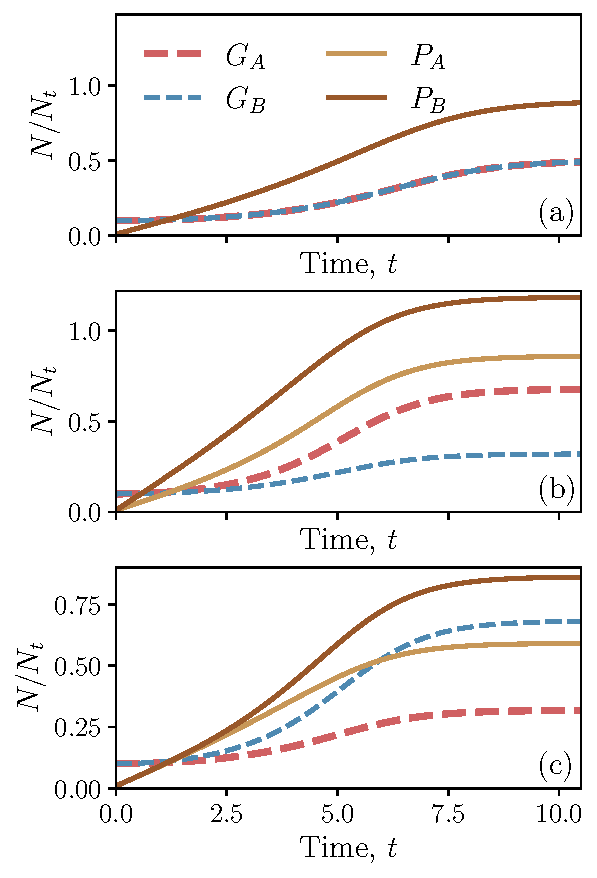
\includegraphics[width=0.5\textwidth]{Figures/pool_model_2sp_1pool_coop.pdf}
    \caption{
        The two-species system where each of the species release public goods $P$ is defined with equations~(\ref{eq:1pool_2sp_cooper}) and calculated for different parameters:
        (a) $\psi=1, \phi=1$, (b) $\psi=1, \phi=2$ and (b) $\psi=2, \phi=1$.
        Here the red lines describes the evolution of the species $G_A$ and blue lines correspond to species $G_B$.
        Light brown curve corresponds to public good released by species $A$ ($P_A$) and brown curve shows public goods produced by species $B$ ($P_B$).
    }
    \label{fig:1pool_2sp_cooper}
    \end{center}
\end{figure}
%
%
%
%
% ================================================================================================
\section{Spatial Limitations}
As described above, the proposed above model operates with the total number of the bacterial counts for different species and states in the system not accounting for their spatial distributions.
Assuming that the bacteria is uniformly distributed we can simplify the problem to the system of the \acp{ode}.
However, in reality spatial effects play significant role for population survival forcing some species develop such competitive mechanism as cell adhesion to surfaces in the areas rich with nutritients~\cite{htuson_bacteriasurface_2013}.
Another mechanism is the motility of bacteria, e.g., the flagellates bacteria as \textit{E. coli} or \textit{B. subtilis} can experience the chemotactic motion of driven by oxygen concentrations~\cite{decoene_microscopic_2011}.
The bacterial social interactions such as releasing the toxins or public goods can also significantly affect the spatial structure of the community~\cite{blanchard_bacterial_2015}.
Therefore, it is rather important to establish the limitations for the model application.\\

- \cite{emonet_agentcell_2005, gorochowski_bsim_2012, li_nufeb_2019, kreft_bacsim_1998}: examples of another toolboxes for bacterial communities modeling (ABM).\\
More about the modelling of the motile bacteria can be seen in works:~\cite{decoene_microscopic_2011, rosser_modelling_2014, sokolov_physical_2012, li_amplified_2008}.
\begin{figure}
    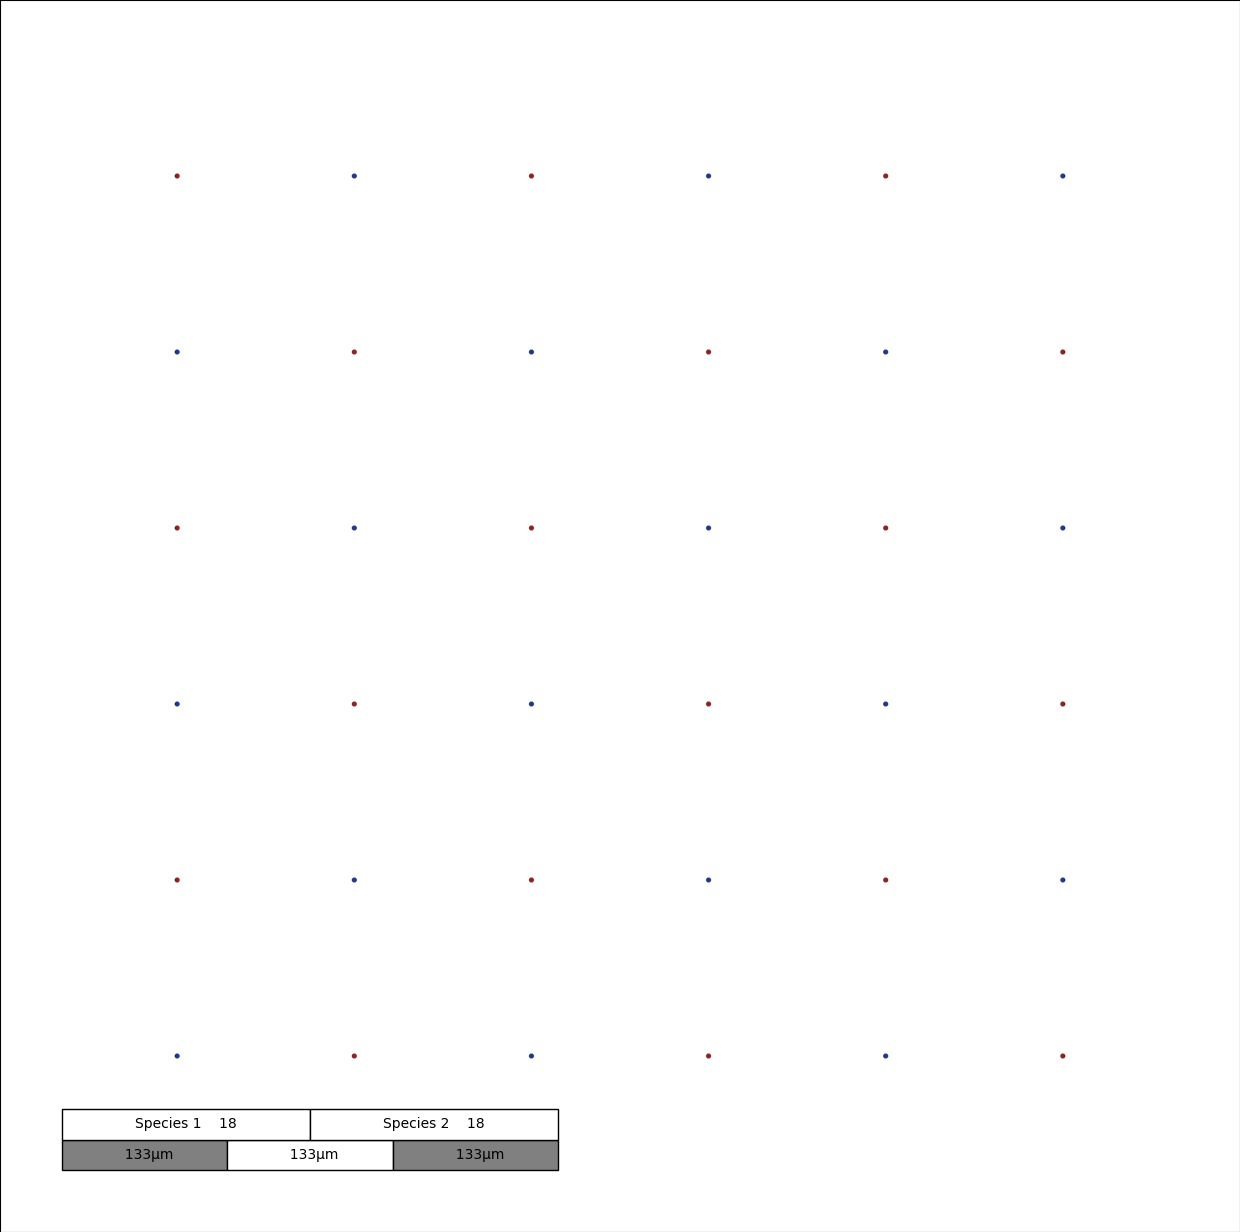
\includegraphics[width=0.49\textwidth]{Figures/snapshot_00000000.png}\hspace{0.02\textwidth}%
    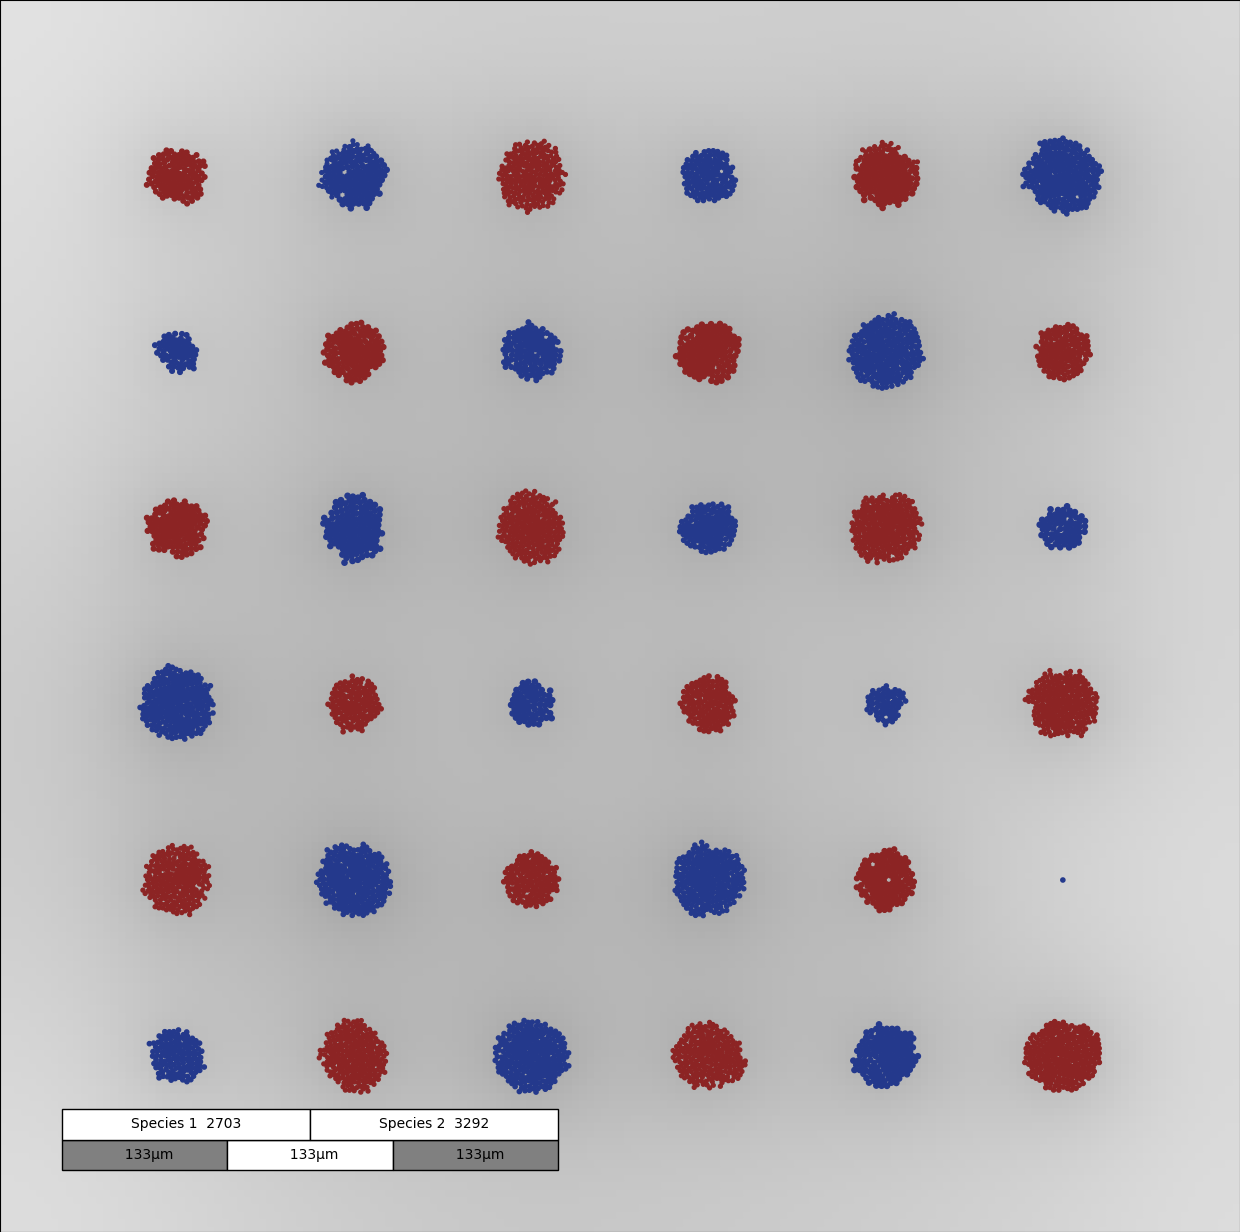
\includegraphics[width=0.49\textwidth]{Figures/snapshot_00006500.png}\vspace{0.02\textwidth}\\
    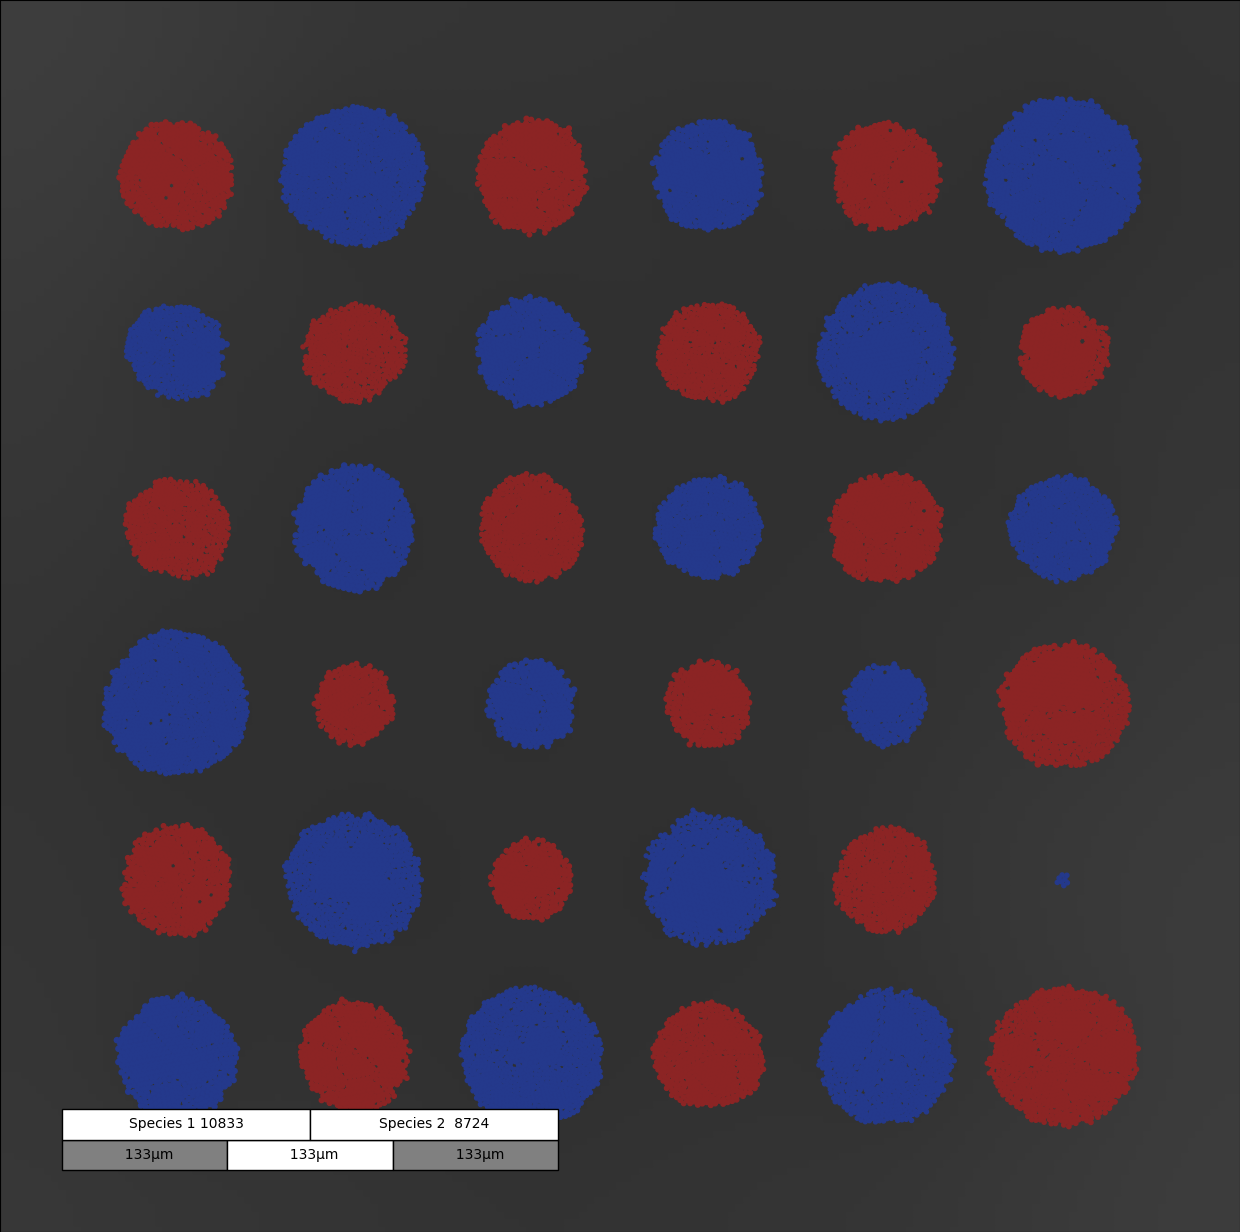
\includegraphics[width=0.49\textwidth]{Figures/snapshot_00013000.png}\hspace{0.02\textwidth}%
    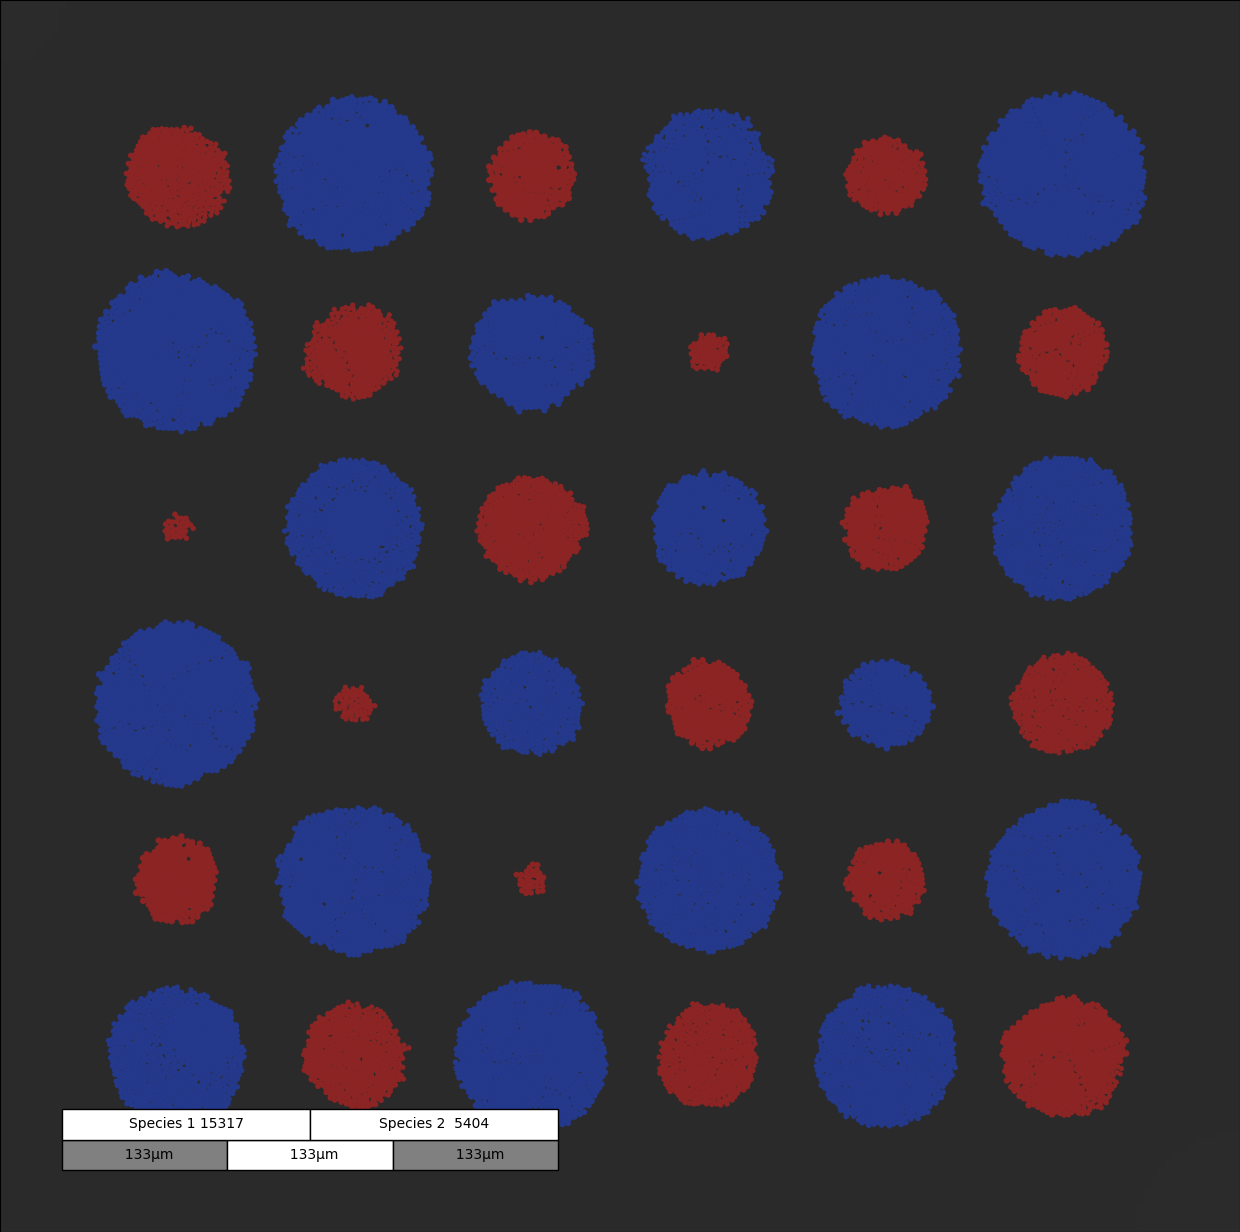
\includegraphics[width=0.49\textwidth]{Figures/snapshot_00020000.png}%
    \caption{}
    \label{fig:spatial-snapshots}
\end{figure}
%
%
\begin{figure}
    \centering
    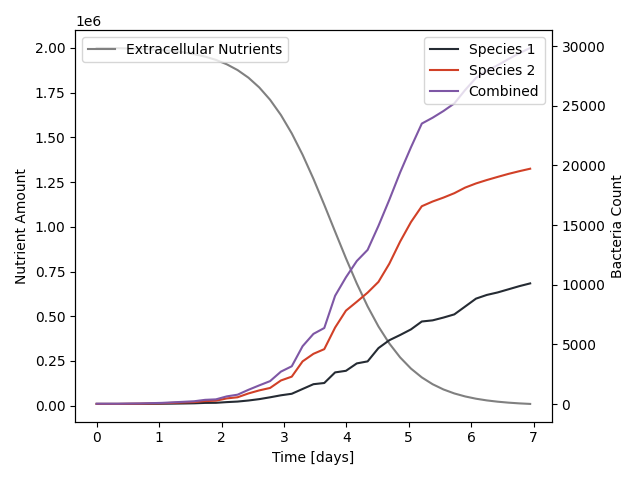
\includegraphics[width=0.6\textwidth]{Figures/spatial_cell_growth.png}
    \caption{}
    \label{fig:spatial-growth-curve}
\end{figure}
%
%
\begin{figure}
    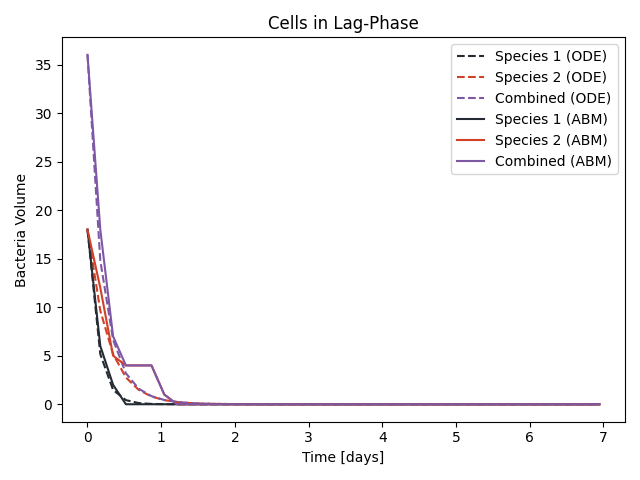
\includegraphics[width=0.5\textwidth]{Figures/lag_phase.png}%
    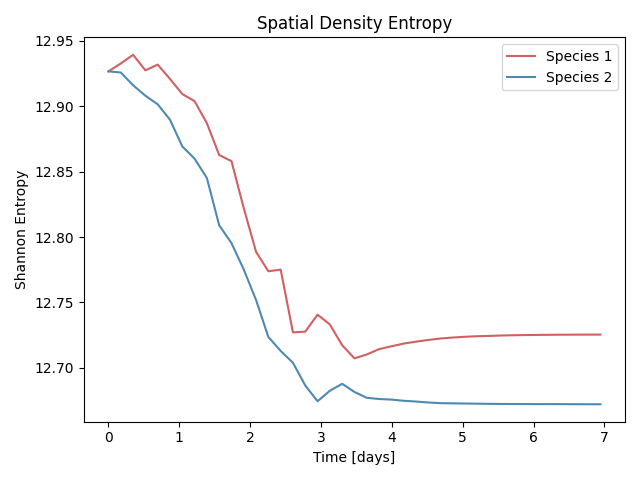
\includegraphics[width=0.5\textwidth]{Figures/entropy.png}
    % TODO difference to pool model
    \caption{}
    \label{fig:spatial-lag-phase-entropy}
\end{figure}
%
%
In general, bacterial communities in 2D can experience collective motion called swarming~\cite{wu_collective_2015}.
Some works modelled 2D motile bacteria:
\begin{itemize}
    \item \cite{decoene_microscopic_2011}: 2D chemotactic self-propelled bacterial motion of the flagellated bacteria (e.g. E. coli, B. subtilis).
    Chemotaxis here was driven by the oxygen concentrations.
    \item \cite{rosser_modelling_2014}: modeling of the bacterial reorintation, rotation.
    \item \cite{sokolov_physical_2012, li_amplified_2008}: modeling of the bacteria using hydrodynamic interactions and Brownian motion.
    Fluctuations in velocity and rotations.
    (\cite{li_amplified_2008}: Brownian motion gives right motion observed using microscopy).
    \item \cite{farrell_mechanically_2013}: 2D modeling using Newtonian dynamics and only mechanical interactions + nutritient diffusion.
    Branching parameter defines diff limits where diffusion dominant and limits growth, and where it's irrelevant.
    Mechanical pressure (due to bacteria-bacteria interactions) affects growth, can limit it.(!!!)
\end{itemize}
%
For simulation results:
\begin{itemize}
    \item \cite{farrell_mechanically_2013}: Showed the influence of mechanic interactions between bacteria in 2D system with bacteria consuming the nutritient.
    The growth of bacterial colonies where non-motile microorganisms replicate and push each other away as they grow.
    Found a transition between two different growth regimes, controlled by the balance between growth and uptake of nutrient:\\
    Exponential growth where diffusion of the nutritient does not play any role. Sublinear growth where growth is limited by nutritient diffusion.
    (Structurally in 2D it's regimes: smooth propagating of bacterial front vs. branching.)
    \item \cite{nagarajan_agent-based_2022-1}: review on the ABM for bacterial population.
    The ABM represent a microbial colony as a group of discrete agents that are governed by a set of rules, where each agent can be an individual cell or a collection of cells.
    Can use citation when talk about general processes we are accounting as growth, uptake of nutritient, production of inhibitor, e.g.,:
    Physical interactions between agents are calculated using excluded volume interactions.
    Chemical interactions as releasing inhibitors are described using concentrations and solved using PDEs.
\end{itemize}
%
To test the spatial limitations of the described above approach consider the system consisting from two bacterial species that can be described by two internal states: lag and growth states. 
Both of these species grow using limiting resource pool $R$ with different growth constants $\alpha$ and different lengths of lag phase determined by parameter $\lambda$.
Moreover, the species 1 is able to release a certain antimicrobial component $I$ that shows inhibitory effect on species 2 (amensalism).
The \acp{ode} the bacterial population can be written as:
\begin{equation}
    \begin{cases}
        \dot{L_1} = -\lambda_1 R L_1\\
        \dot{G_1} = \lambda_1 R L_1 + \alpha_1 R G_1\\
        \dot{L_2} = -\lambda_2 R L_2\\
        \dot{G_2} = \lambda_2 R L_2 + \frac{\alpha_2}{1 + \mu_I I} R G_2\\
    \end{cases}.
    \label{eq:spatial_limit_F}
\end{equation}
%
The microenvironment of our system contains the resource and the inhibitor molecules:
\begin{equation}
    \begin{cases}
        \dot{R} = -\frac{\alpha_1}{N_t} R G_1-\frac{\alpha_2}{(1 + \mu_I I) N_t} R G_2 \\
        \dot{I} = \kappa G_1
    \end{cases}.
    \label{eq:spatial_limit_H}
\end{equation}
%
\begin{table}[H]
    \centering
    \begin{tabular}{ccc}
        \specialrule{.1em}{.01em}{.05em} 
        \textbf{Parameter} \hspace{3mm} & \textbf{Value} \hspace{3mm} & \textbf{Units}\\
        \toprule
        $\lambda_1$ & 0.008  & [time$^{-1}$]                 \\
        $\lambda_2$ & 0.005  & [time$^{-1}$]                 \\
        $\alpha_1$  & 4.0    & [time$^{-1}$]                 \\
        $\alpha_2$  & 5.0    & [time$^{-1}$]                 \\
        $\kappa$    & 0.1    & [(cell $\cdot$ time)$^{-1}$]  \\
        $\mu_I$     & 0.1    & [cell$^{-1}$]                 \\
        $N_t$       & $10^4$ & [cell]                        \\
        \bottomrule
    \end{tabular}
    \caption{The list of the parameters of the system.}
    \label{tab:spatial_limit_param}
\end{table}
%
\begin{table}[H]
    \centering
    \begin{tabular}{ccc}
        \specialrule{.1em}{.01em}{.05em} 
        \textbf{Variable} \hspace{3mm} & \textbf{Initial Value} \hspace{3mm} & \textbf{Units}\\
        \toprule
        $L_1$ & 5.0 & [cell]        \\
        $G_1$ & 0.0 & [cell]        \\
        $L_2$ & 5.0 & [cell]        \\
        $G_2$ & 0.0 & [cell]        \\
        $R$   & 1.0 & [cell/cell]   \\
        $I$   & 0.0 & [cell]        \\
        \bottomrule
    \end{tabular}
    \caption{The list of the initial values of the system.}
    \label{tab:spatial_limit_init}
\end{table}
%
\begin{figure}[H]
    \begin{center}
    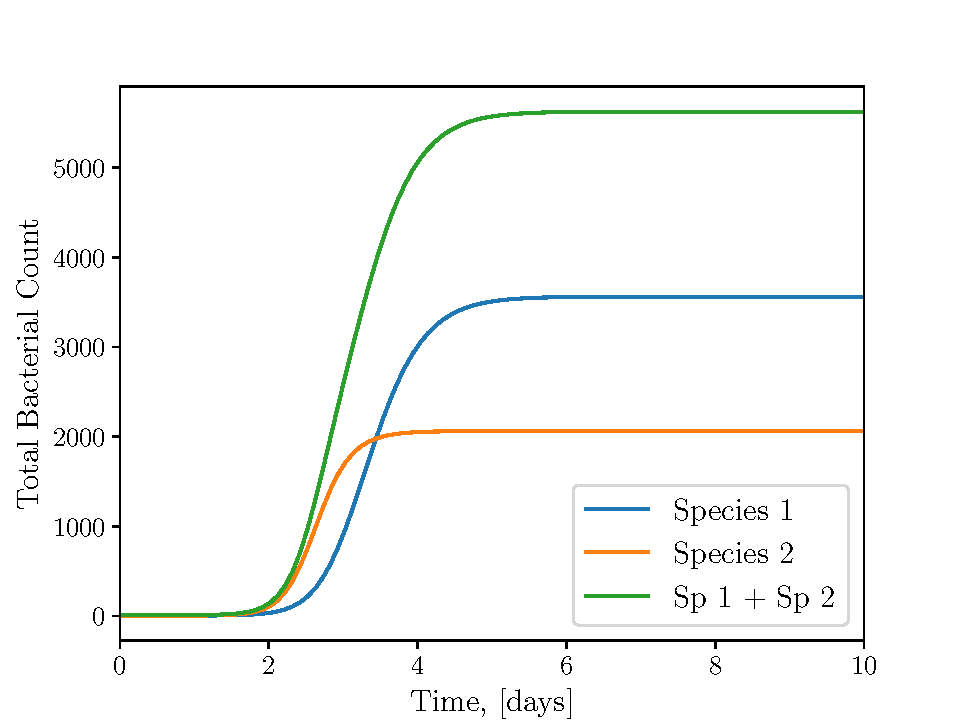
\includegraphics[width=0.6\textwidth]{Figures/pool_model_spatial.pdf}
    \caption{
        The output of the model (\ref{eq:spatial_limit_F}, \ref{eq:spatial_limit_H}) for given parameters and initial valued presented in Tables \ref{tab:spatial_limit_param}, \ref{tab:spatial_limit_init}, respectively.
        The observables of the system are the bacterial count of each species $L+G$ (blue and orange lines) and the total bacterial count of the system (green).
    }
    \label{fig:spatial_limit_plot1}
    \end{center}
\end{figure}
%
\cmtb{The ABM additional parameters $D_R$, $D_I$, $q$ (At which level of $R_i$ cell division happens) and more parameters describing bacterial division.}
%
%
% ================================================================================================
\section{Conclusion}
\newpage
\printbibliography
%
\end{document}
